% This file was created by tikzplotlib v0.9.8.
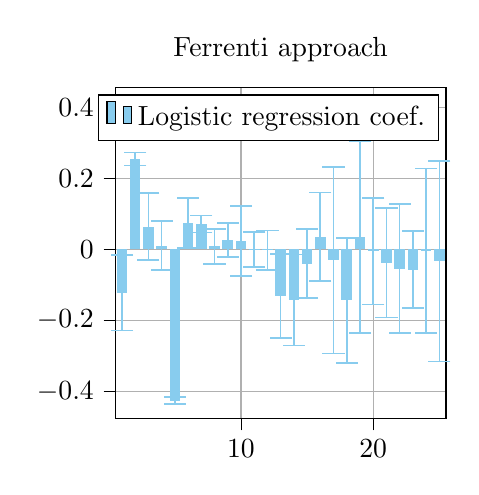
\begin{tikzpicture}

\definecolor{color0}{rgb}{0.533333333333333,0.8,0.933333333333333}

\begin{axis}[
height=2.275590092707901in,
tick align=outside,
tick pos=left,
title={Ferrenti approach},
width=2.275590092707901in,
x grid style={white!69.0196078431373!black},
xmajorgrids,
xmin=0.5, xmax=25.5,
xtick style={color=black},
y grid style={white!69.0196078431373!black},
ymajorgrids,
ymin=-0.476544751038715, ymax=0.454074936965614,
ytick style={color=black}
]
\draw[draw=none,fill=color0] (axis cs:0.6,0) rectangle (axis cs:1.4,-0.123064253300487);
\addlegendimage{ybar,ybar legend,draw=none,fill=color0};
\addlegendentry{Logistic regression coef.}

\draw[draw=none,fill=color0] (axis cs:1.6,0) rectangle (axis cs:2.4,0.254074936965614);
\draw[draw=none,fill=color0] (axis cs:2.6,0) rectangle (axis cs:3.4,0.0637383003312674);
\draw[draw=none,fill=color0] (axis cs:3.6,0) rectangle (axis cs:4.4,0.010153582132699);
\draw[draw=none,fill=color0] (axis cs:4.6,0) rectangle (axis cs:5.4,-0.426544751038715);
\draw[draw=none,fill=color0] (axis cs:5.6,0) rectangle (axis cs:6.4,0.0732655250272369);
\draw[draw=none,fill=color0] (axis cs:6.6,0) rectangle (axis cs:7.4,0.0708059658830058);
\draw[draw=none,fill=color0] (axis cs:7.6,0) rectangle (axis cs:8.4,0.0083798167350135);
\draw[draw=none,fill=color0] (axis cs:8.6,0) rectangle (axis cs:9.4,0.0258456453297823);
\draw[draw=none,fill=color0] (axis cs:9.6,0) rectangle (axis cs:10.4,0.0225188188581133);
\draw[draw=none,fill=color0] (axis cs:10.6,0) rectangle (axis cs:11.4,-0.00133413758881279);
\draw[draw=none,fill=color0] (axis cs:11.6,0) rectangle (axis cs:12.4,-0.00287012168215015);
\draw[draw=none,fill=color0] (axis cs:12.6,0) rectangle (axis cs:13.4,-0.131874778892413);
\draw[draw=none,fill=color0] (axis cs:13.6,0) rectangle (axis cs:14.4,-0.142790669765573);
\draw[draw=none,fill=color0] (axis cs:14.6,0) rectangle (axis cs:15.4,-0.0405779810634156);
\draw[draw=none,fill=color0] (axis cs:15.6,0) rectangle (axis cs:16.4,0.0350731860669815);
\draw[draw=none,fill=color0] (axis cs:16.6,0) rectangle (axis cs:17.4,-0.0311000025985934);
\draw[draw=none,fill=color0] (axis cs:17.6,0) rectangle (axis cs:18.4,-0.14448078918333);
\draw[draw=none,fill=color0] (axis cs:18.6,0) rectangle (axis cs:19.4,0.033212744542326);
\draw[draw=none,fill=color0] (axis cs:19.6,0) rectangle (axis cs:20.4,-0.00593839297518309);
\draw[draw=none,fill=color0] (axis cs:20.6,0) rectangle (axis cs:21.4,-0.0387638090286288);
\draw[draw=none,fill=color0] (axis cs:21.6,0) rectangle (axis cs:22.4,-0.0546645306377975);
\draw[draw=none,fill=color0] (axis cs:22.6,0) rectangle (axis cs:23.4,-0.057269839782401);
\draw[draw=none,fill=color0] (axis cs:23.6,0) rectangle (axis cs:24.4,-0.0041084420499987);
\draw[draw=none,fill=color0] (axis cs:24.6,0) rectangle (axis cs:25.4,-0.0334022639069669);
\path [draw=color0, semithick]
(axis cs:1,-0.229417488366355)
--(axis cs:1,-0.0167110182346182);

\path [draw=color0, semithick]
(axis cs:2,0.23592009450898)
--(axis cs:2,0.272229779422249);

\path [draw=color0, semithick]
(axis cs:3,-0.0305441203965614)
--(axis cs:3,0.158020721059096);

\path [draw=color0, semithick]
(axis cs:4,-0.0595627687059507)
--(axis cs:4,0.0798699329713486);

\path [draw=color0, semithick]
(axis cs:5,-0.436113887749494)
--(axis cs:5,-0.416975614327935);

\path [draw=color0, semithick]
(axis cs:6,0.00255054819934573)
--(axis cs:6,0.143980501855128);

\path [draw=color0, semithick]
(axis cs:7,0.0465056999066113)
--(axis cs:7,0.0951062318594004);

\path [draw=color0, semithick]
(axis cs:8,-0.0409018572150964)
--(axis cs:8,0.0576614906851234);

\path [draw=color0, semithick]
(axis cs:9,-0.0224725241932268)
--(axis cs:9,0.0741638148527915);

\path [draw=color0, semithick]
(axis cs:10,-0.0756353873903538)
--(axis cs:10,0.12067302510658);

\path [draw=color0, semithick]
(axis cs:11,-0.0502658861107364)
--(axis cs:11,0.0475976109331108);

\path [draw=color0, semithick]
(axis cs:12,-0.0580334518860479)
--(axis cs:12,0.0522932085217476);

\path [draw=color0, semithick]
(axis cs:13,-0.250619578161296)
--(axis cs:13,-0.0131299796235295);

\path [draw=color0, semithick]
(axis cs:14,-0.270974675652396)
--(axis cs:14,-0.0146066638787493);

\path [draw=color0, semithick]
(axis cs:15,-0.137679517728949)
--(axis cs:15,0.0565235556021181);

\path [draw=color0, semithick]
(axis cs:16,-0.0895883476180547)
--(axis cs:16,0.159734719752018);

\path [draw=color0, semithick]
(axis cs:17,-0.293950085783651)
--(axis cs:17,0.231750080586464);

\path [draw=color0, semithick]
(axis cs:18,-0.319655037072536)
--(axis cs:18,0.0306934587058758);

\path [draw=color0, semithick]
(axis cs:19,-0.236206876473511)
--(axis cs:19,0.302632365558163);

\path [draw=color0, semithick]
(axis cs:20,-0.155739313287969)
--(axis cs:20,0.143862527337602);

\path [draw=color0, semithick]
(axis cs:21,-0.192747588063431)
--(axis cs:21,0.115219970006173);

\path [draw=color0, semithick]
(axis cs:22,-0.235981974229328)
--(axis cs:22,0.126652912953733);

\path [draw=color0, semithick]
(axis cs:23,-0.16625366350342)
--(axis cs:23,0.0517139839386183);

\path [draw=color0, semithick]
(axis cs:24,-0.235550284144142)
--(axis cs:24,0.227333400044145);

\path [draw=color0, semithick]
(axis cs:25,-0.315874390637381)
--(axis cs:25,0.249069862823448);

\addplot [semithick, color0, mark=-, mark size=4, mark options={solid}, only marks]
table {%
1 -0.229417488366355
2 0.23592009450898
3 -0.0305441203965614
4 -0.0595627687059507
5 -0.436113887749494
6 0.00255054819934573
7 0.0465056999066113
8 -0.0409018572150964
9 -0.0224725241932268
10 -0.0756353873903538
11 -0.0502658861107364
12 -0.0580334518860479
13 -0.250619578161296
14 -0.270974675652396
15 -0.137679517728949
16 -0.0895883476180547
17 -0.293950085783651
18 -0.319655037072536
19 -0.236206876473511
20 -0.155739313287969
21 -0.192747588063431
22 -0.235981974229328
23 -0.16625366350342
24 -0.235550284144142
25 -0.315874390637381
};
\addplot [semithick, color0, mark=-, mark size=4, mark options={solid}, only marks]
table {%
1 -0.0167110182346182
2 0.272229779422249
3 0.158020721059096
4 0.0798699329713486
5 -0.416975614327935
6 0.143980501855128
7 0.0951062318594004
8 0.0576614906851234
9 0.0741638148527915
10 0.12067302510658
11 0.0475976109331108
12 0.0522932085217476
13 -0.0131299796235295
14 -0.0146066638787493
15 0.0565235556021181
16 0.159734719752018
17 0.231750080586464
18 0.0306934587058758
19 0.302632365558163
20 0.143862527337602
21 0.115219970006173
22 0.126652912953733
23 0.0517139839386183
24 0.227333400044145
25 0.249069862823448
};
\end{axis}

\end{tikzpicture}
